\documentclass[12pt,a4paper,openany]{book}

\input{C:/Users/serru/Documents/Codes/LaTeX/Environnement_package.tex}
\input{C:/Users/serru/Documents/Codes/LaTeX/Environnements_settings.tex}
\input{C:/Users/serru/Documents/Codes/LaTeX/Environnement_theorems.tex}

\setcounter{tocdepth}{4}
\sloppy

\title{}
\author{Serrurot Gabin\\
BTS SNIR}
\date{\today}

\begin{document}

\sloppy

\vspace*{\stretch{1}}
\begin{minipage}{0.9\linewidth}
\rule{\linewidth}{0.5mm}\\[0.2cm]
\huge\bfseries
\begin{center}
Mathématiques
\end{center}
\rule{\linewidth}{0.5mm}\\[0.2cm]
\maketitle
\end{minipage}
\vspace*{\stretch{1}}

\newpage

\tableofcontents

\newpage

\chapter{Trigonométrie}

\section{Cercle trigonométrique}

\begin{figure}[!h]
\begin{center}
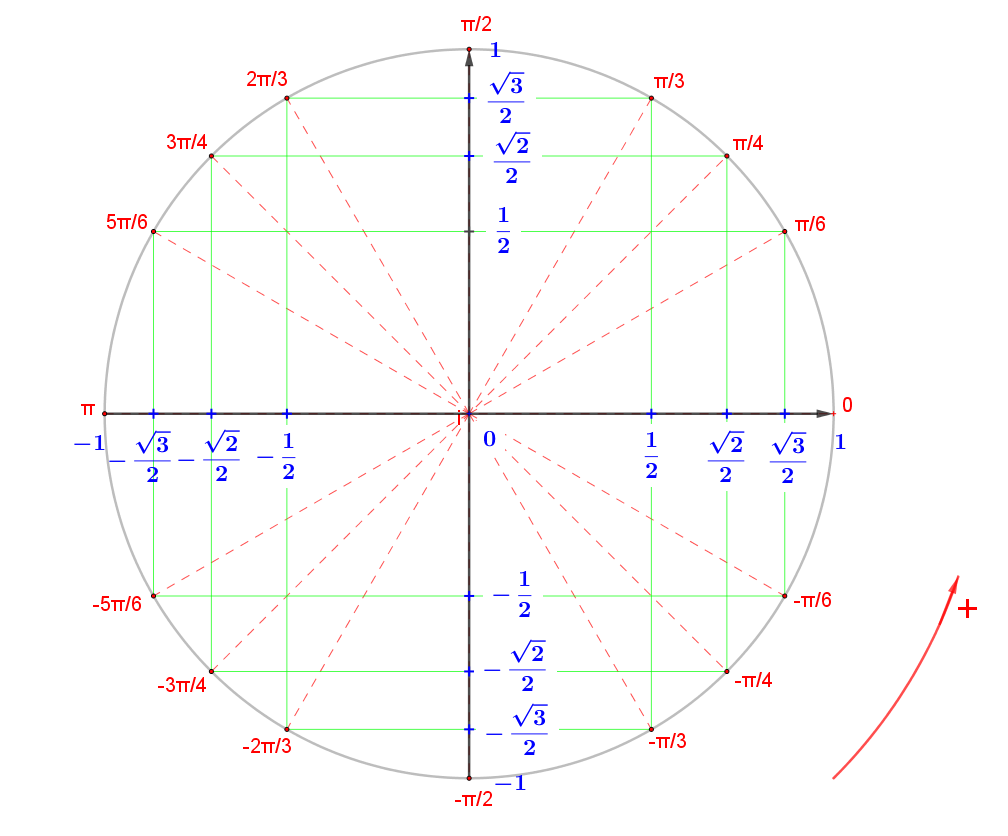
\includegraphics[scale=0.5]{Images/cercleTrigonometrique.png} 
\caption{Image montrant le cercle trigonométrique ainsi que la position des valeurs remarquables du tableau~\ref{tableauAnglesRemarquables}.}
\label{cercleTrigo}
\end{center}
\end{figure}

\section{Fonctions sinus et cosinus}

\paragraph{Cosinus} Nous avons plusieurs relations remarquables pour la fonction $ cos(x) $:
\begin{align}
cos(x) & = cos(-x)\\
cos(\pi - x) & = -cos(x) = cos(\pi + x)
\end{align}

Nous pouvons associer à cette fonction la fonction $ arccos(x) $ qui est sa fonction réciproque. Elle est définie sur $ [0; \pi] $.

\paragraph{Sinus} Nous avons plusieurs relations remarquables pour la fonction $ sin(x) $:
\begin{align}
sin(x) & = -sin(x)\\
sin(\pi - x) & = sin(x)\\
sin(\pi + x) & = -sin(x)
\end{align}

Nous pouvons associer à cette fonction la fonction $ arcsin(x) $ qui est sa fonction réciproque. Elle est définie sur $ [-\frac{\pi}{2}; \frac{\pi}{2}] $.

\section{Fonction tangente}

\chapter{Généralités sur les fonctions}

\section{Fonctions usuelles}

\section{Dérivées de fonctions usuelles}

\section{Calculer une dérivée de fonctions usuelles}

\end{document}